\section{Simulation Environment}
In this work, we introduce a differentiable simulation environment tailored for DLO manipulation. We implemented the simulator using the Taichi~\citep{hu2019taichi,hu2020difftaichi} programming language and integrated it into Genesis~\citep{Genesis} to build a versatile benchmark for DLO manipulation. Our simulator models a broad range of DLO's behaviors and its interactions with other rigid or soft bodies.

\subsection{DLO Modeling}
Following the classic discrete elastic rod (DER)~\citep{bergou2008discrete, bergou2010discrete} methods, DLO-Lab represents a deformable linear object $\rmX$ as a centerline specified by a set of $\text{N}_v$ vertices and a set of $\text{N}_e$ adapted, orthonormal frames attached to each edge:
\begin{align}
\begin{split}
    \rvx &= \{\rvx_i|\rvx_i\in\sR^3\}\\
    \rvd &= 
    \left\{(\rvd_1, \rvd_2, \rvd_3)^j| \rvd_1, \rvd_2, \rvd_3 \in \mathrm{SO(3)}\right\},
\end{split}
\end{align}
where $0\leq i\leq \text{N}_v$ and $0 \leq j \leq \text{N}_e$. The term \emph{adapted} means that $\rvd^j_3$ lies along the edge given by the adjacent vertices, $\rve^j=\rvx_{j+1}-\rvx_j$, and $\rvd^j_3\equiv\rve^j/|\rve^j|$.
During forward simulation, the internal interaction of DLOs is modeled by the potential energy $U(\rmX^t)$, where $\rmX^t$ denotes the state variables (\ie, vertex states $\rvx^t$ and frame states $\rvd^t$) of the DLO at time $t$. Concretely, the potential energy is composed of stretching energy $U_s(\rvd^t)$, bending energy $U_b(\rvx^t)$, and twisting energy $U_t(\rvx^t)$. We calculate the derivatives $\partial U/\partial \rmX^t$ and employ a standard symplectic Euler solver for time stepping. In addition, we model the bending plasticity by introducing a yield threshold $\sigma_y$ and a creep rate $r_c$, which are used to adjust the rest curvatures when the yield constraint is violated. Furthermore, we model the frictional contact behavior between DLOs using position-based dynamics~\citep{muller2007position}, which simplifies the process of solving complex and computationally expensive non-linear equations typically required by preventative methods like IPC~\citep{li2020incremental,li2021codimensional}. See Appendix~\ref{sec:DLORepr} for more details about the representation of DLOs used in this work.

\subsection{Coupling Implementation}

\begin{figure*}[t]
    \begin{center}
        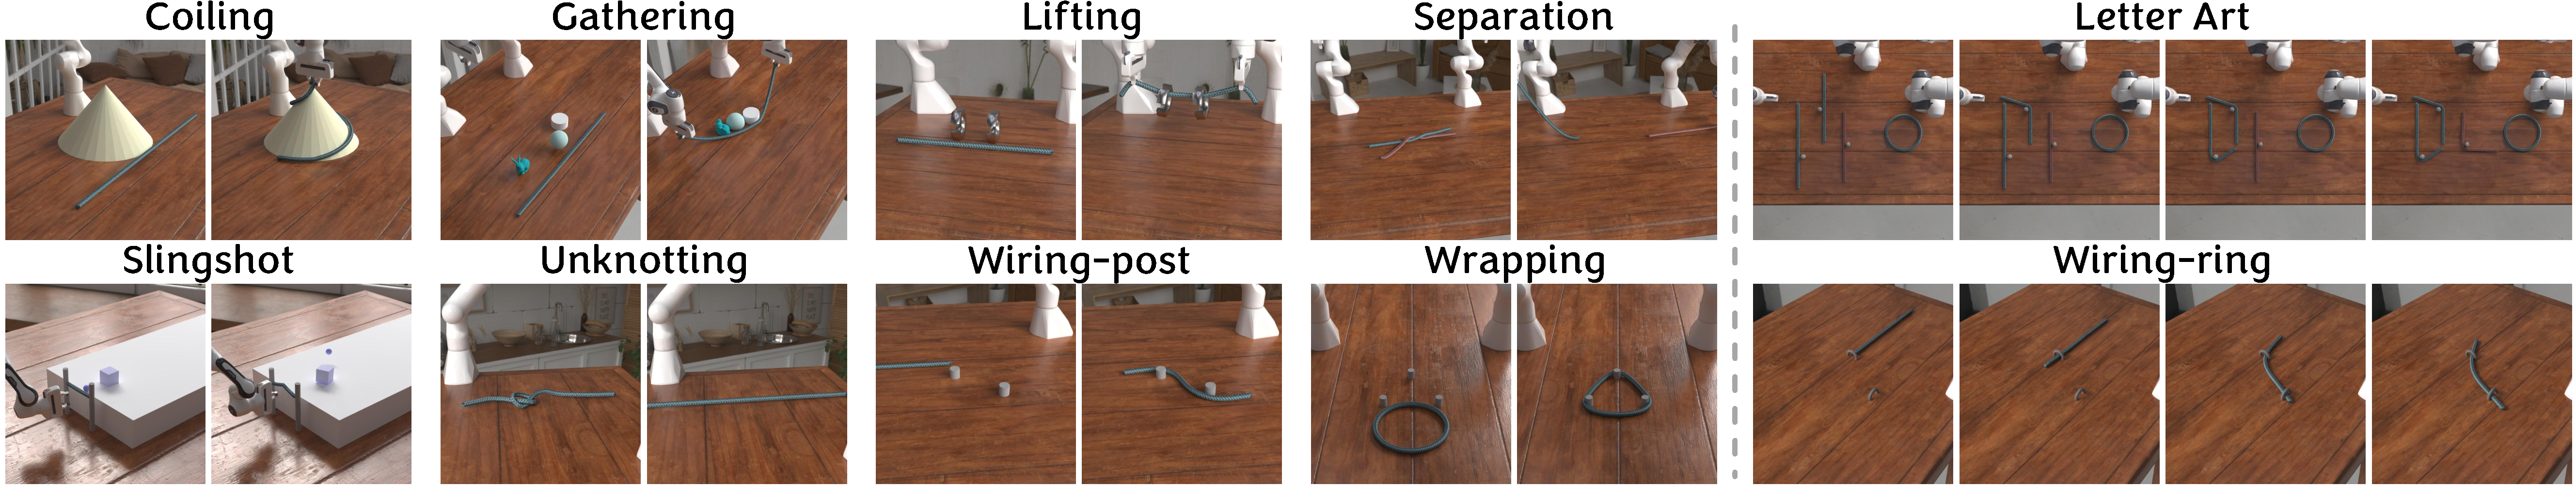
\includegraphics[width=\linewidth]{figs/tasks_v2.pdf}
    \end{center}
    \vspace{-4mm}
    \caption{\textbf{Task illustration.} Our benchmark comprises 10 manipulation tasks: 8 fixed-horizon tasks shown on the left and 2 long-horizon tasks displayed on the right. The initial and desired goal states for each task are illustrated.}
    \label{fig:tasks}
    \vspace{-4mm}
\end{figure*}

\paragraph{Rigid Body} We adopt the rigid solver from Genesis~\cite{Genesis} and implement a two-way coupling scheme between DLOs and rigid bodies. The rigid solver models each rigid geometry as a time-varying signed distance field (SDF).
At each simulation step, we calculate the penetration depth $d$ of each rigid geometry for every sampled position $\rvp$ along the centerline of the DLO: $d(\rvp)=r(\rvp)-\mathrm{SDF}(\rvp)$, where $r$ is the radius. Rather than a hard binary contact, we use a soft-coupling approach where an exponential influence factor $f_i$, determined by a tunable softness parameter $\epsilon_s$, is calculated based on the penetration depth: $f_i = \min \big(\exp(d/\epsilon_s),1\big)$. When $f_i$ exceeds a predefined threshold (0.1 as used in this work), we resolve the collision using an impulse-based response. The contact normal is derived from the gradient of the SDF, and we decompose the relative velocity between the sampled location of DLO and the contact point on the rigid body into normal and tangent components.
This allows us to apply a standard restitution model to the normal component and a friction model to the tangential component. We calculate the change in the momentum at $\rvp$ and apply an equal and opposite reaction force back to the rigid body to ensure momentum conservation. Additionally, to stabilize the grasp with a rigid gripper, we identify the nearest vertices in contact with the manipulator and flag them as kinematic for the current time step. This prevents the DLO's internal position-based collision handling scheme from generating conflicting updates, ensuring that the DLO deforms compliantly around the gripper.
\vspace{-4mm}

\paragraph{Soft Body} To simulate the complex interactions between DLOs and other volumetric materials, such as fluids and elasto-plastic objects, we propose a two-way coupling scheme between our DLO solver and the Material Point Method (MPM)~\citep{jiang2016material,hu2018moving} solver implemented in Genesis~\cite{Genesis}. We treat the interaction as a collision process mediated by the MPM Eulerian grid. Specifically, within the MPM grid operation loop, we detect collisions between active grid nodes and the DLO's geometry, represented by both its vertices and edges. When a grid node penetrates the DLO's collision volume, we calculate a repulsive impulse based on the relative velocity, surface normal, and material properties, such as restitution coefficients and local mass ratios. This impulse is applied symmetrically to ensure momentum conservation. It instantly updates the grid node's velocity to resolve the penetration of the soft body, while simultaneously applying an equal and opposite reaction force to the corresponding DLO vertices via atomic operations. This method facilitates stable, immediate bidirectional feedback between the discrete DLO elements and the continuum-based soft material within a single simulation step, enabling the simulation of multi-material phenomena, as illustrated in~\Cref{fig:teaser}(c).


\subsection{Gradient Back-propagation}

Our simulator, implemented with Taichi~\citep{hu2019taichi,hu2020difftaichi}, benefits from its automatic differentiation (autodiff) to compute numerical gradients. However, a key challenge in achieving full differentiability in the simulation is enabling gradient flow throughout time. A naïve solution is to maintain a record of the simulation states at every timestep. Nevertheless, tasks in DLO-Lab often require thousands of simulation steps, rendering the naïve solution infeasible given limited GPU memory. To address this issue, we drew inspiration from FluidLab~\citep{xianfluidlab} and implemented gradient checkpointing to enable gradient backpropagation over the entire simulation trajectory. Specifically, to allow backpropagation through simulations of arbitrary length without being limited by GPU memory, we use gradient checkpointing. During the forward pass, we compute the simulation trajectory in segments. At the end of each segment, we cache a single state checkpoint in CPU memory and discard the intermediate GPU states. For the backward pass, we iterate through these checkpoints in reverse order. For each checkpoint, we rerun the forward simulation for the local segment to reconstruct the necessary computational graph, then perform the backward pass. This method balances the memory cost of storing the entire simulation history with the computational cost of recomputing small portions of the trajectory, keeping the memory requirement independent of the simulation horizon.
